%% BioMed_Central_Tex_Template_v1.06
%%                                      %
%  bmc_article.tex            ver: 1.06 %
%                                       %

%%IMPORTANT: do not delete the first line of this template
%%It must be present to enable the BMC Submission system to
%%recognise this template!!

%%%%%%%%%%%%%%%%%%%%%%%%%%%%%%%%%%%%%%%%%
%%                                     %%
%%  LaTeX template for BioMed Central  %%
%%     journal article submissions     %%
%%                                     %%
%%          <8 June 2012>              %%
%%                                     %%
%%                                     %%
%%%%%%%%%%%%%%%%%%%%%%%%%%%%%%%%%%%%%%%%%


%%%%%%%%%%%%%%%%%%%%%%%%%%%%%%%%%%%%%%%%%%%%%%%%%%%%%%%%%%%%%%%%%%%%%
%%                                                                 %%
%% For instructions on how to fill out this Tex template           %%
%% document please refer to Readme.html and the instructions for   %%
%% authors page on the biomed central website                      %%
%% http://www.biomedcentral.com/info/authors/                      %%
%%                                                                 %%
%% Please do not use \input{...} to include other tex files.       %%
%% Submit your LaTeX manuscript as one .tex document.              %%
%%                                                                 %%
%% All additional figures and files should be attached             %%
%% separately and not embedded in the \TeX\ document itself.       %%
%%                                                                 %%
%% BioMed Central currently use the MikTex distribution of         %%
%% TeX for Windows) of TeX and LaTeX.  This is available from      %%
%% http://www.miktex.org                                           %%
%%                                                                 %%
%%%%%%%%%%%%%%%%%%%%%%%%%%%%%%%%%%%%%%%%%%%%%%%%%%%%%%%%%%%%%%%%%%%%%

%%% additional documentclass options:
%  [doublespacing]
%  [linenumbers]   - put the line numbers on margins

%%% loading packages, author definitions

\documentclass[twocolumn]{bmcart}% uncomment this for twocolumn layout and comment line below
%\documentclass{bmcart}

%%% Load packages
%\usepackage{amsthm,amsmath}
%\RequirePackage{natbib}
%\RequirePackage[authoryear]{natbib}% uncomment this for author-year bibliography
%\RequirePackage{hyperref}
\usepackage[utf8]{inputenc} %unicode support
%\usepackage[applemac]{inputenc} %applemac support if unicode package fails
%\usepackage[latin1]{inputenc} %UNIX support if unicode package fails
\usepackage{float}
%\usepackage[showframe]{geometry}
%\usepackage{lipsum}
\usepackage{hyperref}
%\usepackage{multicols}{2}
%%%%%%%%%%%%%%%%%%%%%%%%%%%%%%%%%%%%%%%%%%%%%%%%%
%%                                             %%
%%  If you wish to display your graphics for   %%
%%  your own use using includegraphic or       %%
%%  includegraphics, then comment out the      %%
%%  following two lines of code.               %%
%%  NB: These line *must* be included when     %%
%%  submitting to BMC.                         %%
%%  All figure files must be submitted as      %%
%%  separate graphics through the BMC          %%
%%  submission process, not included in the    %%
%%  submitted article.                         %%
%%                                             %%
%%%%%%%%%%%%%%%%%%%%%%%%%%%%%%%%%%%%%%%%%%%%%%%%%


\def\includegraphic{}
\def\includegraphics{}
\usepackage{graphicx}



%%% Put your definitions there:
\startlocaldefs
\endlocaldefs

\usepackage{float}
%%% Begin ...
\begin{document}


%%% Start of article front matter
\begin{frontmatter}

\begin{fmbox}
\dochead{Software}

%%%%%%%%%%%%%%%%%%%%%%%%%%%%%%%%%%%%%%%%%%%%%%
%%                                          %%
%% Enter the title of your article here     %%
%%                                          %%
%%%%%%%%%%%%%%%%%%%%%%%%%%%%%%%%%%%%%%%%%%%%%%

\title{SEPIA: Simulation-based Evaluation of Prioritization Algorithms}

%%%%%%%%%%%%%%%%%%%%%%%%%%%%%%%%%%%%%%%%%%%%%%
%%                                          %%
%% Enter the authors here                   %%
%%                                          %%
%% Specify information, if available,       %%
%% in the form:                             %%
%%   <key>={<id1>,<id2>}                    %%
%%   <key>=                                 %%
%% Comment or delete the keys which are     %%
%% not used. Repeat \author command as much %%
%% as required.                             %%
%%                                          %%
%%%%%%%%%%%%%%%%%%%%%%%%%%%%%%%%%%%%%%%%%%%%%%

\author[
   addressref={aff1},
   noteref={n1},
]{\inits{KA}\fnm{Kimberly} \snm{Almaraz}}
\author[
   addressref={aff1},
   noteref={n1},
]{\inits{TJ}\fnm{Tyler} \snm{Jang}}
\author[
   addressref={aff1},
   noteref={n1},
]{\inits{ML}\fnm{McKenna} \snm{Lewis}}
\author[
   addressref={aff1},
   noteref={n1},
]{\inits{TN}\fnm{Titan} \snm{Ngo}}
\author[
   addressref={aff1},
   noteref={n1},
]{\inits{MS}\fnm{Miranda} \snm{Song}}
\author[
   %addressref={aff1},
   %noteref={n1},
   email={niema@ucsd.edu}
]{\inits{NM}\fnm{Niema} \snm{Moshiri}}
%%%%%%%%%%%%%%%%%%%%%%%%%%%%%%%%%%%%%%%%%%%%%%
%%                                          %%
%% Enter the authors' addresses here        %%
%%                                          %%
%% Repeat \address commands as much as      %%
%% required.                                %%
%%                                          %%
%%%%%%%%%%%%%%%%%%%%%%%%%%%%%%%%%%%%%%%%%%%%%%

\address[id=aff1]{%                           % unique id
  \orgname{Department of Computer Science and Engineering, University of California San Diego}, % university, etc
  \street{9500 Gilman Dr.},                     %
  \postcode{92093}                                % post or zip code
  \city{La Jolla},                              % city
  \cny{USA}                                    % country
}


%%%%%%%%%%%%%%%%%%%%%%%%%%%%%%%%%%%%%%%%%%%%%%
%%                                          %%
%% Enter short notes here                   %%
%%                                          %%
%% Short notes will be after addresses      %%
%% on first page.                           %%
%%                                          %%
%%%%%%%%%%%%%%%%%%%%%%%%%%%%%%%%%%%%%%%%%%%%%%

\begin{artnotes}
%\note{Sample of title note}     % note to the article
\note[id=n1]{Equal contributor} % note, connected to author
\end{artnotes}

%\end{fmbox}% comment this for two column layout

%%%%%%%%%%%%%%%%%%%%%%%%%%%%%%%%%%%%%%%%%%%%%%
%%                                          %%
%% The Abstract begins here                 %%
%%                                          %%
%% Please refer to the Instructions for     %%
%% authors on http://www.biomedcentral.com  %%
%% and include the section headings         %%
%% accordingly for your article type.       %%
%%                                          %%
%%%%%%%%%%%%%%%%%%%%%%%%%%%%%%%%%%%%%%%%%%%%%%

\begin{abstractbox}

\begin{abstract} % abstract
\parttitle{Background}
The ability to prioritize people living with HIV by risk of future transmissions could aid public health officials in optimizing epidemiological intervention. While methods exist to perform such prioritization based on molecular data, their effectiveness and accuracy are poorly understood, and it is unclear how one can directly compare the accuracy of different methods. We introduce SEPIA (Simulation-based Evaluation of PrIoritization Algorithms), a novel simulation-based framework for determining the effectiveness of prioritization algorithms.
SEPIA expands on prior related work
%in simulation-based comparisons of HIV care prioritization techniques
by defining novel metrics of effectiveness with which to compare prioritization techniques as well as by creating a simulation-based tool with which to perform such effectiveness comparisons.
Under several metrics of effectiveness that we propose, we
%utilize various properties of the simulated contact networks and transmission histories to
compare two existing prioritization approaches: one phylogenetic (ProACT) and one distance-based (growth of HIV-TRACE transmission clusters).
%We use FAVITES, an epidemic simulation tool, to generate this simulated data.
%We personally used SEPIA to analyze the results of both distance-based and phylogenetic prioritization methods.

\parttitle{Results}
%Text for this section.
%Upon testing SEPIA on two different prioritization algorithms, ProACT (phylogenetic-based) and HIV-Trace (distance-based), we found that,
Using all proposed metrics, ProACT consistently slightly outperformed the transmission cluster growth approach. However, both methods consistently performed just marginally better than random, suggesting that there is significant room for improvement in prioritization tools.

\parttitle{Conclusion}
We hope that, by providing ways to quantify the effectiveness of prioritization methods in simulation, SEPIA will aid researchers in developing novel tools for prioritizing people living with HIV by risk of future transmissions.

\end{abstract}

%%%%%%%%%%%%%%%%%%%%%%%%%%%%%%%%%%%%%%%%%%%%%%
%%                                          %%
%% The keywords begin here                  %%
%%                                          %%
%% Put each keyword in separate \kwd{}.     %%
%%                                          %%
%%%%%%%%%%%%%%%%%%%%%%%%%%%%%%%%%%%%%%%%%%%%%%

\begin{keyword}
\kwd{SEPIA}
\kwd{HIV}
\kwd{Prioritization}
\kwd{Metrics}
\kwd{Simulation-based Evaluation}
\kwd{FAVITES}
\kwd{Phylogenetic}
\end{keyword}

% MSC classifications codes, if any
%\begin{keyword}[class=AMS]
%\kwd[Primary ]{}
%\kwd{}
%\kwd[; secondary ]{}
%\end{keyword}

\end{abstractbox}

\end{fmbox}% uncomment this for two column layout

\end{frontmatter}

%%%%%%%%%%%%%%%%%%%%%%%%%%%%%%%%%%%%%%%%%%%%%%
%%                                          %%
%% The Main Body begins here                %%
%%                                          %%
%% Please refer to the instructions for     %%
%% authors on:                              %%
%% http://www.biomedcentral.com/info/authors%%
%% and include the section headings         %%
%% accordingly for your article type.       %%
%%                                          %%
%% See the Results and Discussion section   %%
%% for details on how to create sub-sections%%
%%                                          %%
%% use \cite{...} to cite references        %%
%%  \cite{koon} and                         %%
%%  \cite{oreg,khar,zvai,xjon,schn,pond}    %%
%%  \nocite{smith,marg,hunn,advi,koha,mouse}%%
%%                                          %%
%%%%%%%%%%%%%%%%%%%%%%%%%%%%%%%%%%%%%%%%%%%%%%

%%%%%%%%%%%%%%%%%%%%%%%%% start of article main body
% <put your article body there>

%%%%%%%%%%%%%%%%
%% Background %%
%%
%
%\section*{Content}
%Text and results for this section, as per the individual journal's instructions for authors. %\cite{koon,oreg,khar,zvai,xjon,schn,pond,smith,marg,hunn,advi,koha,mouse}

\section*{Background}
%Human immunodeficiency virus (HIV) is one of the world's most deadly infectious diseases, significantly impacting regions including sub-Saharan Africa, Asia, the Pacific, and Latin America \cite{cdc1}. In 2019, there were 38.0 million people living with HIV globally, with 1.7 million people newly infected and 690,000 HIV-related deaths \cite{who}. 
Molecular data gathered on human immunodeficiency virus (HIV) is useful for understanding the systems of epidemic spread of HIV. Such understanding can better allow us to intervene and treat high-risk groups of individuals. Methods of epidemic intervention include treatments such as antiretroviral therapy (ART) and awareness programs \cite{cdc2}. Adherence to ART can cause viral suppression in people living with HIV and significantly reduce their risk of transmission, making ART distribution a potentially effective approach to combating the spread of HIV. However, a major issue for public health officials is the limited amount of resources available and how to allocate them. 
%Thus, they need to turn to tools that determine which high-risk individuals they ought to prioritize.
%Given the scale of this epidemic and the difficulties in tracing viral transmissions, however, there are limited resources available, and these limited resources need to be allocated effectively. The deployment of these can be optimized using tools that evaluate the transmission of HIV and determine which individuals are most at risk. \cite{wertheim2018growth}.

% is "specific mutated variant of HIV" correct terminology?
%Analyses of viral sequences are often used to track the evolution and spread of the virus, with each genetic sample representing a specific mutated variant of HIV in an HIV-positive individual \cite{wertheim2018growth}. These viral sequences are usually taken from individuals starting ART and seeking treatment at medical facilities.
In many parts of the world, when testing and treating individuals living with HIV, it has become standard practice to record various metadata on the patients, including viral genomic sequences (often of the \textit{pol} and \textit{gag} regions). This information is often used to determine groups of individuals with high risk of future transmission, which can help public health officials to better allocate limited resources \cite{wertheim2018growth}. 
The prioritization of people living with HIV can be explored through a computational framework: given a list of individuals along with metadata and viral sequences, order the individuals in descending order of inferred risk of future transmission.
%Researchers have developed tools that each take in a list of such sequences and output a ranking that prioritizes individuals based on each individual's relative risk of transmitting HIV to others. With inferred data from these tools, healthcare officials can better determine where to direct epidemiological intervention and limited resources \cite{wertheim2018growth}.

Molecular epidemiology provides a natural framework for prioritizing individuals from viral sequence data. Currently, the standard approach is to use HIV-TRACE \cite{pond2018hivtrace} to infer transmission clusters based on pairwise distances between sequences, monitor the growth of the transmission clusters over time, and prioritize individuals in descending order of transmission cluster growth. ProACT \cite{moshiri2019ProACT}, on the other hand, is a prioritization approach that utilizes properties of a phylogeny inferred from the viral sequences.

The following questions naturally arise: how well does a given prioritization method perform, and which method is superior in specific contexts? With real-world data, the ground truth of who transmitted to whom is typically unavailable or error-prone. Further, even \textit{with} a known transmission history, it is unclear how to quantify effectiveness: do we count the number of transmissions from a single individual? Do we count the total number of transmissions in a transmission chain seeded from a single individual? Rather than the transmission network itself, perhaps we are interested in properties of the underlying contact network (e.g. prioritize individuals with large numbers of social contacts)? Thus, it is unclear how to even quantitatively assess the performance of different prioritization methods.

% short summary of sepia, details of how it works in detail should be elsewhere  in the methods section if at all, reword for better grammar
To address this open problem, we introduce SEPIA (Simulation-based Evaluation of PrIoritization Algorithms), a novel simulation-based framework for measuring the effectiveness of prioritization algorithms.
Previously, in Moshiri \textit{et al.} (2021)~\cite{moshiri2019ProACT}, two prioritization algorithms were compared with respect to effectiveness, but the comparisons were limited to a simulated epidemic dataset modeling the San Diego HIV epidemic between 2005 and 2014.
Like this prior work, SEPIA utilizes simulated epidemic data, such as those generated by FAVITES \cite{moshiri2018favites} or PANGEA.HIV.sim \cite{ratmann2016phylogenetic}, to define a ground truth with which prioritization methods can be directly compared.
However, SEPIA expands on this prior work by generalizing the task of prioritization effectiveness comparison and further exploring the mathematical meaning of ``effectiveness'' by defining 6 metrics of effectiveness, each inspired by properties of epidemics that are inherently of interest to public health officials for intervention.
Specifically,
the user runs a prioritization method on a simulated dataset;
then, given the prioritization and the simulated dataset, SEPIA will measure the effectiveness of the prioritization using the metrics defined below.
%The results produced by SEPIA can then be used to characterize the performance of a single prioritization approach on different epidemic scenarios (represented by different simulated data sets) as well as to directly compare the performance of multiple prioritization approaches. 

%SEPIA will take two different sets of data for its input. The first input will be the prioritization results ran on simulated data and the  second input will be the simulated data gathered from FAVITES. The first thing SEPIA will do is assign a priority value based off the simulated data. This priority value will then be given a rank determined from the metric that was used. Each person in the data will have a priority value and this value becomes a rank on how much each person should be prioritized. This rank gets compared to the algorithms ordering on how will it prioritizes each person. This comparison is done with the Kendall Tau calculation. When compared SEPIA will output a coefficient between the ranked values and the algorithms ordering.%


\section*{Methods}
Given a prioritization, SEPIA computes an effectiveness score according to one of several metrics we have implemented, defined below.
\newline
\begin{itemize}

\item \textbf{Metric 1: Direct Transmissions} This metric aims to quantify the direct impact of each individual \textit{u} on the spread of the virus within a population by counting the total number of individuals to whom \textit{u} directly transmitted.\newline

\item \textbf{Metric 2: Transmission Rate} This metric aims to quantify the rate of transmission of each individual \textit{u}, giving higher values to those who transmitted to the most individuals over shorter and more recent time periods.
Specifically, for each individual \textit{u}, we produce a step function representing the number of transmissions from individual \textit{u} over time (Fig. 1) starting from the time of \textit{u}'s first transmission and ending at the termination of the simulation, and we measure the slope of a regression line inferred from the step graph. Because the horizontal axes of all individuals' step graphs are bounded by the same simulation end time, an individual with more frequent and recent outgoing transmissions with respect to the end-time will have a steeper slope and will thus be assigned a higher value.\newline

%------FIGURE 1
\begin{figure}[h!]
\centering
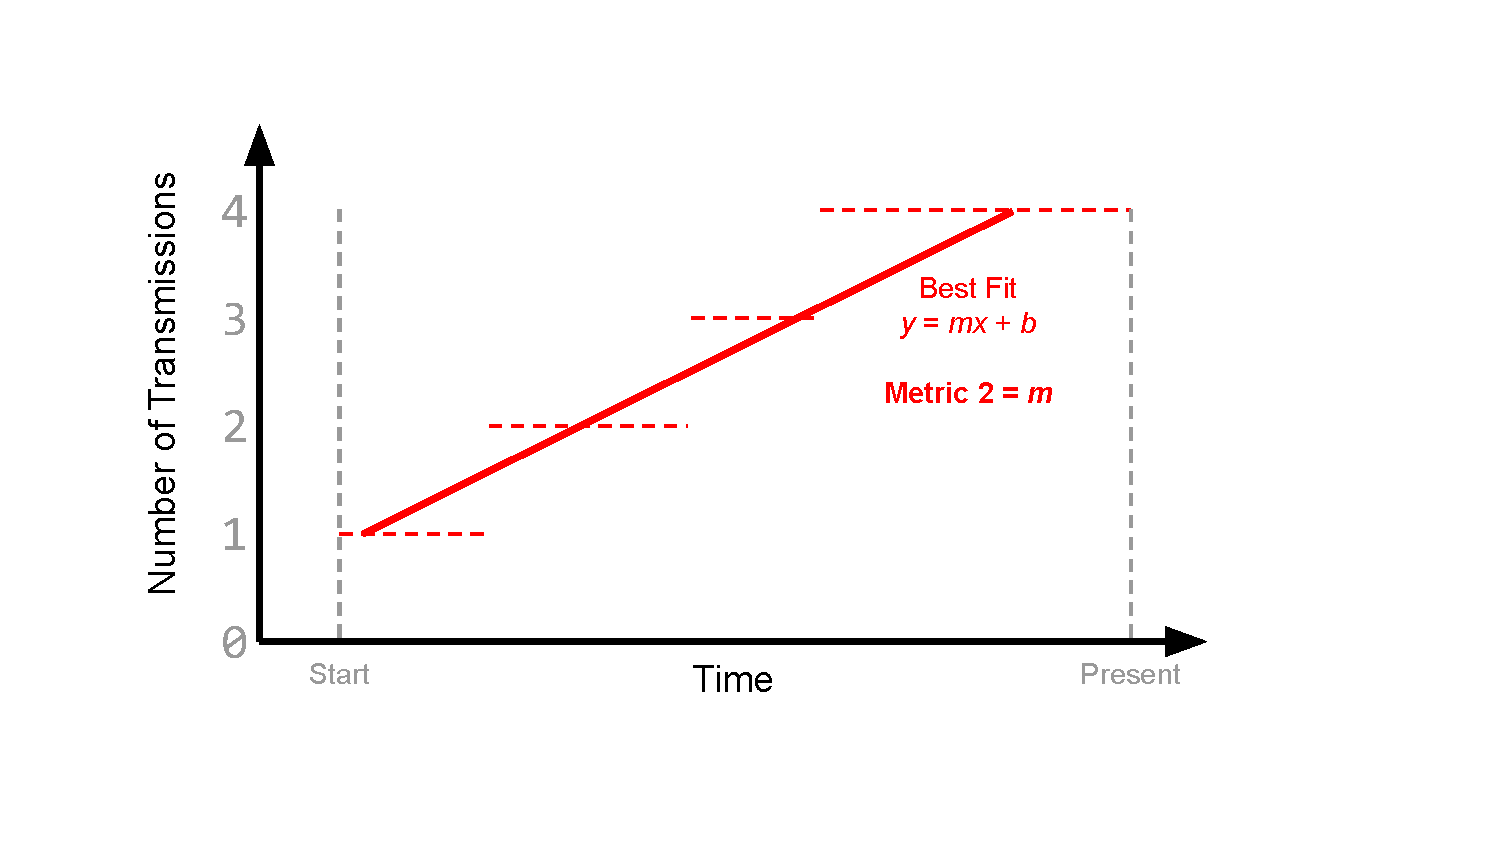
\includegraphics[width=0.45\textwidth]{Figures/Fig1.pdf}
\caption{
\newline 
Metric 2. Because Person B has transmitted to more individuals more recently than has Person A, the regression line of Person B has a larger slope.
}
\end{figure}

%------FIGURE 
%\begin{figure}[h!]
%\centering
%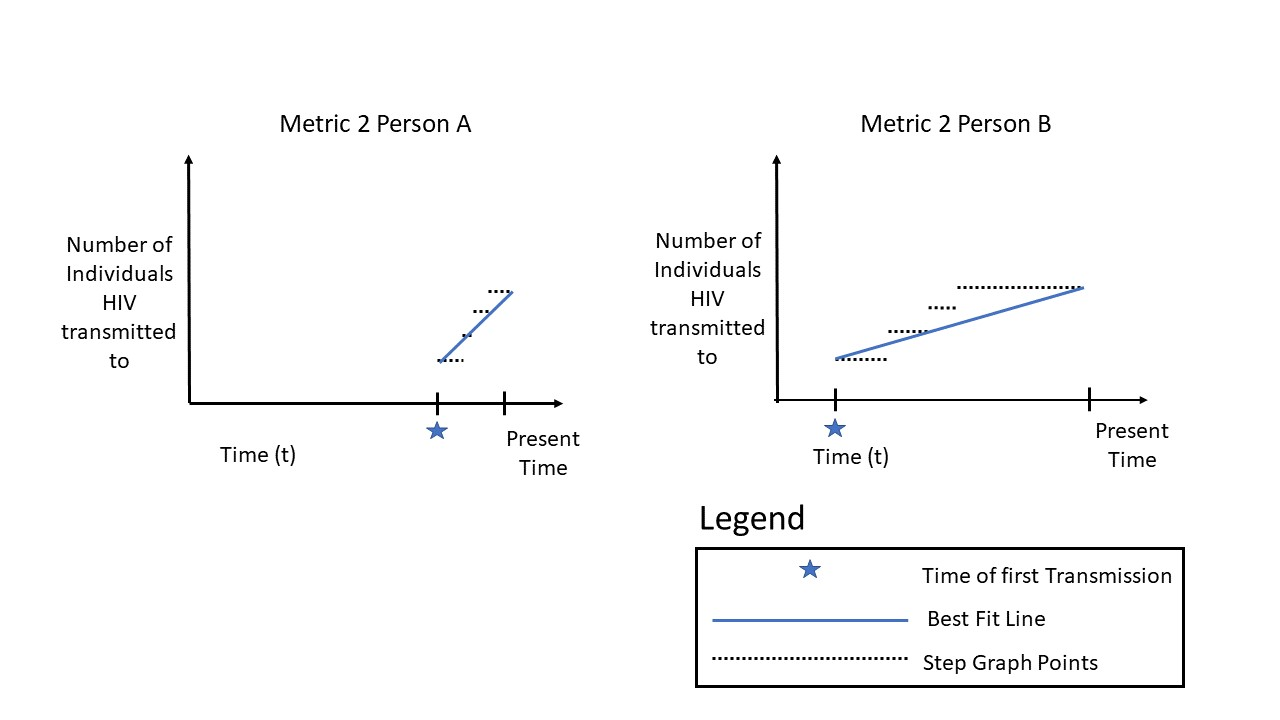
\includegraphics[scale=0.25]{Figures/Metric 2.jpg}
%\caption{Above, we illustrate example plots for two %individuals, where one  individual transmitted HIV to %others more recently (\textit{2a}) and the other %individual transmitted HIV others longer ago %(\textit{2b}), with the graph on the left having a %greater slope and thus representing an individual with %greater priority.}
%\end{figure}
%------FIGURE  END
\item \textbf{Metric 3: Indirect Transmissions} This metric expands on Metric 1 in order to quantify an individual's broader impact on the community. Specifically, for an individual \textit{u}, we count the number of individuals who were infected by somebody who was infected by \textit{u} (i.e., we count the secondary transmissions of \textit{u}).\newline

\item \textbf{Metric 4: Direct and Indirect Transmissions} This is the sum of Metrics 1 and 3.
\newline

\item \textbf{Metric 5: Number of Contacts} Metric 5 measures each individual's total number of contacts in the underlying contact network.
\newline

\item \textbf{Metric 6: Number of Contacts and Transmissions} This is the sum of Metrics 1 and 5.\newline

\end{itemize}

% Why we use simulated data
%To construct optimal orderings for evaluating prioritization algorithms, it is necessary to have knowledge of all possible person-to-person HIV transmissions and sexual contacts within a given time frame. This is captured through the contact network and the transmission network. The contact network represents all interactions between individuals (with respective time points) through which HIV could have been transmitted. The transmission network represents all actual occurrences (with respective time points) of HIV transmission. At first, we considered using real-world data to evaluate prioritization techniques. However, given the real-world limitations of data collection, the contact and transmission networks assembled from actual data are typically inaccurate or incomplete. Without a true transmission history, we cannot determine a potential optimal ordering that prioritizes individuals in a data set by their risk of transmission. Thus, in order to obtain a complete transmission history, simulated data must be utilized to evaluate prioritization algorithms.

% Specifically, how we get our simulated data (FAVITES)
%SEPIA utilizes FrAmework for VIral Transmission and Evolution Simulation (FAVITES) to generate simulated data that can be used to test prioritization algorithms. FAVITES simulates end-to-end HIV epidemics, including full contact and transmission networks (\textit{Figure 2}). It accounts for both random processes and user-selected parameters such as population size, rate of starting ART, and rate of adherence to ART \cite{moshiri2018favites}. FAVITES simulates a realistic epidemic in which individuals start and adhere to ART in a consistent and life-like manner.

%figure 2
\begin{figure}[!h]
\centering
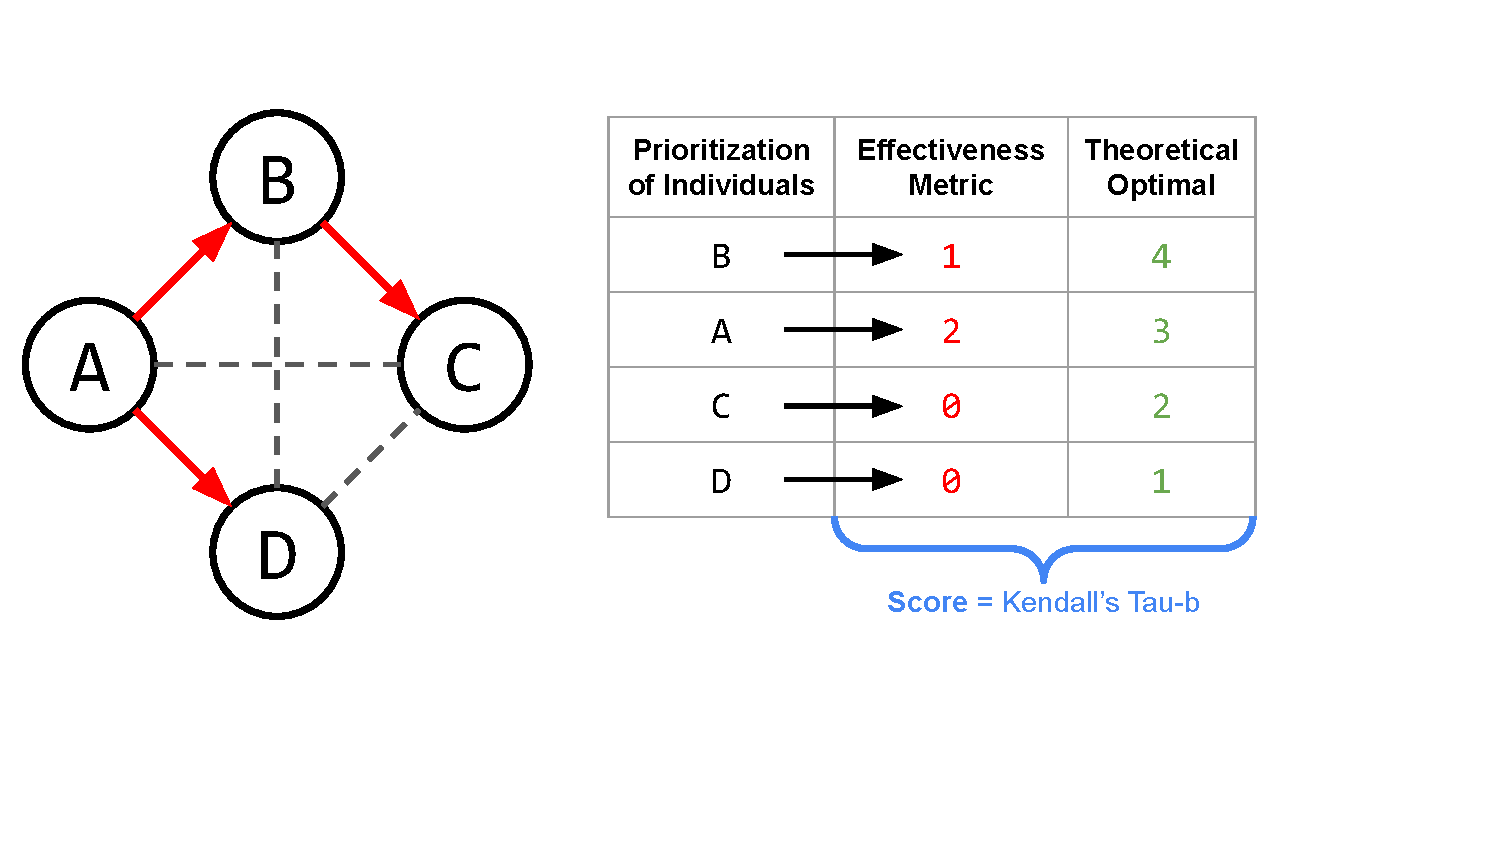
\includegraphics[width=0.45\textwidth]{Figures/Fig2.pdf}
\caption{Flowchart of the different stages of the SEPIA workflow. The first two boxes indicate SEPIA's two required Inputs: the simulated data and a prioritization of the individuals in the simulated data. In Steps 1 and 2, each individual in the prioritization is paired with a count value, calculated by a selected metric in the simulated data. In Step 3, we calculate the Kendall Tau-b correlation coefficient, our Output, between these count values and the theoretically optimal ordering of count values.}
\end{figure}

Given a prioritization and the simulated data from which the prioritization was produced, for a given selected metric, SEPIA will compute a value for each individual in the prioritization (Fig. 2). Given a prioritization with a computed metric value for each individual, SEPIA then constructs an ``optimal'' prioritization by simply sorting the individuals in descending order of metric value. To compare the user-given prioritization against the optimal, SEPIA computes the Kendall Tau-b rank correlation coefficient \cite{kendall1938new}.

We used SEPIA to compare the effectiveness of two molecular epidemiological prioritization methods. One approach is to use HIV-TRACE to infer transmission clusters from pairwise distances of viral sequences, monitor the growth of the transmission clusters over time, and prioritize individuals in descending order of transmission cluster growth. The other approach is ProACT \cite{moshiri2019ProACT}, a method that utilizes properties of a phylogeny inferred from the viral sequences. We used a simulated dataset produced by FAVITES to emulate the HIV pandemic in San Diego between 2005 and 2014 \cite{moshiri2018favites}. The simulated datasets vary the expected degree in the contact network $\left(E_d\right)$, the rate at which individuals begin ART $\left(\lambda_+\right)$, and the rate at which individuals stop adhering to ART $\left(\lambda_-\right)$.

%------FIGURE 2
%\begin{figure}[h!]
%\centering
%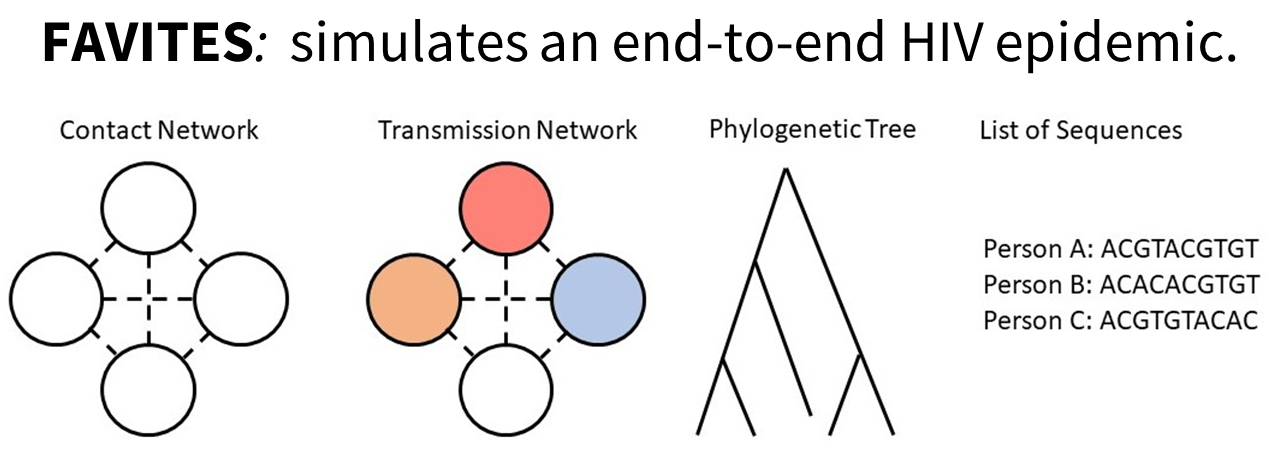
\includegraphics[scale=0.225]{Figures/FAVITES.png}
%\caption{FAVITES simulates an end-to-end HIV epidemic. It generates four different representations of a simulated epidemic as contact networks, transmission networks, phylogenetic trees, and lists of sequences.}
%\end{figure}

% Simulated data as input to prioritization algorithm and SEPIA
%The workflow for evaluating a prioritization algorithm begins with passing in simulated viral sequences as inputted into the prioritization algorithm (\textit{Figure 1}). On the other hand, SEPIA takes in contact and/or transmission networks from the same simulated epidemic data set. 

% Introduces metrics and count values
%To measure the efficacy of a prioritization algorithm across various environmental conditions, SEPIA offers six distinct metrics to generate optimal orderings. Each metric defines a unique way of calculating count values for individuals by analyzing a defined characteristic in the simulated data over a specified time period, such that individuals with higher count values will have higher priority in the ordering. 

% Optimal ordering explanation
%The optimal ordering is a list of individuals sorted, in descending order, by their risk of transmitting HIV. Individuals who are more likely to transmit HIV based on prior history in the form of contact and transmission networks should be more highly prioritized.

%To generate the optimal ordering, SEPIA defines the six following metrics to calculate individuals' count values:


%------FIGURE 4a&b
%\begin{figure}[h!]
%\centering
%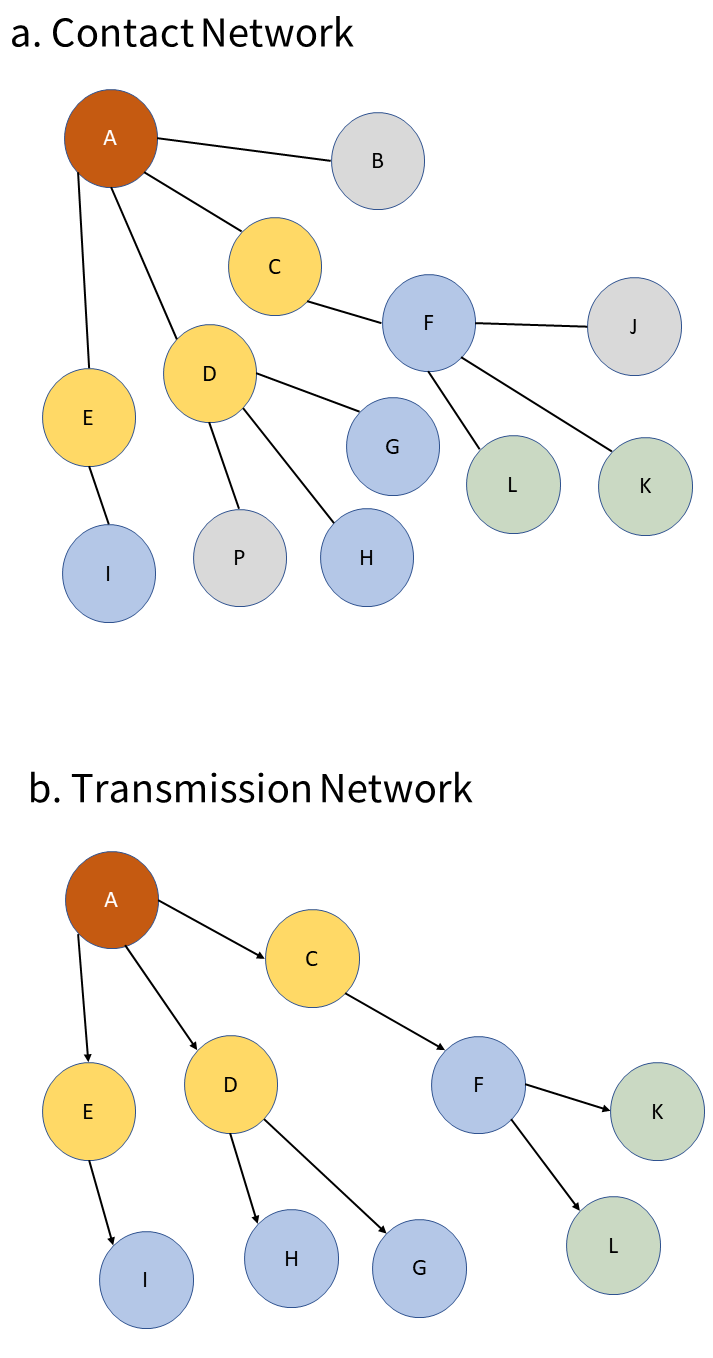
\includegraphics[scale=0.35]{Figures/SEPIA networks.png}
%\caption{
%\newline
%a. Let Nodes represent individuals in the epidemic, and let each undirected edge represent sexual contact between two persons such that there is a chance for HIV transmission. This information is used by several metrics, including Metric 5, which determines an individual's count by the number of contacts they have. If Node A is being observed in Metric 5, Node A's count would be 4 due to it having 4 undirected edges. 
%\newline\newline
%b. Let Nodes represent individuals in the epidemic, and let each directed edge represent the transmission of HIV from one person to another. This information is used by several metrics, including Metric 1 and Metric 3. Under Metric 1, Node A would have a count of 3 (total count of yellow Nodes), while under Metric 3, Node A would have a count of 4 (total count of blue nodes).
%}
%\end{figure}
%------FIGURE 4 END


%LIST OF METHODS-------------------------------------------------


%------FIGURE 
%\begin{figure}[h!]
%\centering
%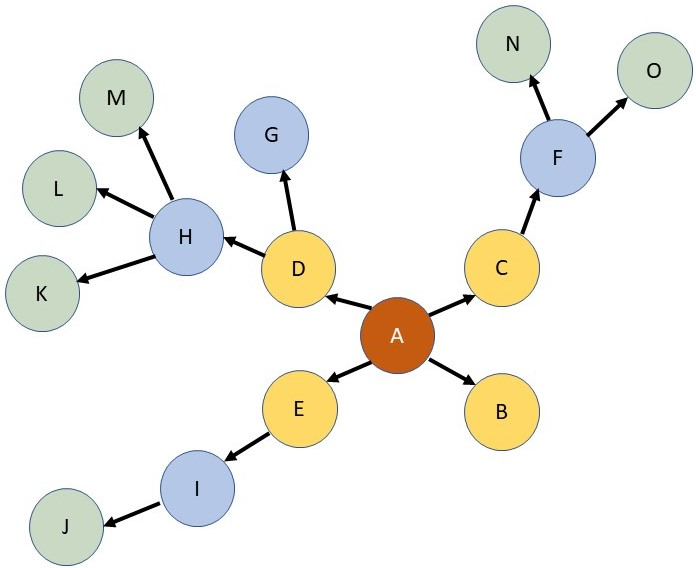
\includegraphics[scale=0.43]{Figures/transmission network.jpg}
%\caption{An illustration of how individuals are %counted in Metric 1, Metric 3, and Metric 4.
%Let every node in the graph represent an HIV positive individual, with the red node representing the individual \textit{H} we are calculating a count value for, and let every directed edge between nodes represent a transmission of HIV from one individual to another.
%To calculate the count for \textit{H}, \textbf{Metric 1} would count all orange nodes.
%\textbf{Metric 3} would count all blue nodes, while \textbf{Metric 4} merges these two metrics by counting all orange nodes \textit{and} all blue nodes.} 
%\end{figure}
%------FIGURE  END

%END LIST OF METHODS-----------------------------------------------------

%------FIGURE 3c END
% Prioritization algorithm - output comparison - final output
%The prioritization algorithm's output, an ordering that ranks individuals by their likelihood of being the next outgoing transmission, is compared to the ordering produced by SEPIA from the same simulated data set using a specified metric. This comparison outputs a Kendall Tau-b correlation coefficient as the final measure of the prioritization algorithm's efficacy. 

%The Kendall Tau-b correlation coefficient is calculated with a variety of orderings generated by our metrics for given algorithms. The framework can provide a greater understanding of how optimal a particular ordering is by comparing an algorithm's ordering of individuals to the optimal ordering for a given metric. The following are our metrics for calculating count values paired with each individual in order to determine optimal orderings:
%In the final step of all six of our metrics, the list of individuals' counts, sorted in descending order of priority, represents an optimal ordering that is compared to the ordering outputted by the prioritization algorithm being evaluated \textit{X}. This comparison is done by calculating the Kendall Tau-b correlation coefficient between these two lists. This coefficient describes how closely-related the solution's ordering is to the most optimal (sorted) ordering \cite{kendall1938new}. A value of 1.0 indicates perfect correlation, or greatest possible accuracy, and a value of 0 indicates no correlation, or an accuracy no better than a randomly-generated ordering.


% TODO **Figure X. Effectiveness of prioritization methods.** Kendall Tau-b values are shown for each of the effectiveness metrics across all tested experimental conditions.
% E_d denotes the expected number of contacts per individual, \lambda_+ denotes the rate at which individuals begin ART, and \lambda_- denotes the rate at which individuals stop ART.
\section*{Results}
%We tested SEPIA on two algorithms, HIV-Trace and ProACT, which have different approaches to determining individual priorities \cite{wertheim2018growth, moshiri2019ProACT}. (\textit{Figure 5}) shows the combined results of all 6 metrics. These figures show the results of running ProACT and HIV-Trace on SEPIA using simulated data from FAVITES many different data sets under different conditions. 
%TODO

As can be seen in Figure 3, ProACT consistently outperformed HIV-TRACE transmission cluster growth using all metrics on all simulation conditions. However, both tools consistently had Tau-b scores marginally higher than 0, implying that they are performing only marginally better than a random ordering.
% Explain what happens as Ed, lamda_, and lambda+ changes
As the rate of starting ART $\left(\lambda_+\right)$ increases, the rate of stopping ART $\left(\lambda_-\right)$ increases, and the expected degree $\left(E_d\right)$ increases (i.e., as the outbreak spreads more quickly), ProACT's performance with respect to metrics 5 and 6 seems to increase slightly. Otherwise, both ProACT and HIV-TRACE transmission cluster growth seem to perform fairly consistently across experimental conditions.


%As more people stop adhering to ART $\left(\lambda_-\right)$,
%Pro. On the other hand, HIV-Trace's ordering does not show such an increase in the positive correlation with the optimal ordering, showing a decreased positive correlation with larger values of $\lambda_-$. The difference in performance between HIV-Trace and ProACT is most pronounced for $\lambda_-$ when $\lambda_-= 4x$, where the correlation difference between HIV-Trace and ProACT is the greatest.

%As the rate people start ART $\left(\lambda_+\right)$ increases, meaning there are more people in the simulated data that begin treatment, we see the correlation between ProACT's ordering compared to the optimal ordering decrease slightly. The difference between the performance of ProACT's ordering and HIV-Trace's ordering also decreases as $lambda_+$ increases. This is most prevalent when $\lambda_+ = 4$, as the difference in performance between ProACT's ordering and HIV-Trace's ordering is the least.

%The number of expected sexual contacts per person $\left(E_d\right)$, which would affect the rate the virus could spread, did not have consistent effects on the correlation between HIV-Trace's ordering or ProACT's ordering with the optimal ordering. Whether $E_d = 10$ or $E_d = 20$, there appears to be little difference in the performance of either HIV-Trace or ProACT. When $E_d = 30$, there is a slight decrease in the performance in ProACT compared to the optimal ordering in Metric 1 to Metric 4, however, the performance increases in Metric 5 and Metric 6. Thus, the effect of $E_d$ is not consistent across all metrics.

%The figures shows that the results of Metric 1 look very similar to the results of Metric 2 and Metric 4. This is likely due to the data set containing few or no individual with a significantly higher amount of transmissions than any other individual in the given range of time, as well as low spread in the times of transmission. It is likely that if one individual has a high number of direct transmissions, their step count would also be very steep. However, the data set does not contain such an individual. Thus, Metric 2 will act relatively similarly to Metric 1 in the sense that it will simply count the number of direct transmissions when no individual has a relatively higher amount of direct transmissions more recently than any other. Metric 4 is based on the sum of Metric 1 and Metric 3, and in our data it is likely that Metric 1 has a larger weight than Metric 3 in determining a tool's ordering. Thus, this would likely explain why the results of Metric 4 look similar to the results of Metric 1. 

\section*{Discussion}
Across all defined metrics and all considered simulation conditions, ProACT consistently outperformed prioritization by HIV-TRACE transmission cluster growth. However, both approaches consistently performed just marginally better than a random ordering, implying that there is room for significant improvement in the realm of HIV prioritization.
%that while ProACT does perform slightly better than HIV-Trace, neither model performs significantly better than random when predicting the next individual to become HIV positive in any environmental condition. Both these algorithms' Kendall Tau-b correlation coefficients are near 0.00 in all metrics, which means they perform approximately as well as a random ordering in comparison to the optimal ordering of individuals who ought to be prioritized. 

% TODO, spread??, verify w Niema, do we need this paragraph?
%The figures shows that the results of Metric 1 look very similar to the results of Metric 2. This is likely due to the data set containing no individual with a significantly greater amount of transmissions in the given range of time, as well as low spread in the times of transmission. It is likely that if one individual has a high number of direct transmissions, their step count would also be very steep. Thus, Metric 2 will act relatively similarly to Metric 1 in the sense that it will simply count the number of direct transmissions when no individual has a relatively higher amount of direct transmissions more recently than any other.

It must be noted that, while we aimed to provide generalized results by varying key simulation parameters, the simulated epidemics are specifically modeled after the HIV epidemic in San Diego. Molecular epidemiologists will need to assess prioritization techniques using simulated datasets representative of the pathogens and communities in which they are interested.

We hope that SEPIA will enable researchers to quantify and assess the effectiveness of different prioritization approaches in order to select the best existing prioritization method for their communities, develop new prioritization methods that improve upon existing ones, and, ultimately, maximize the impact of the limited resources available to public health officials.
% \begin{figure}[h!]  %Figure 6
% \centering
% \title\textbf{Metric 1}\par\medskip
% 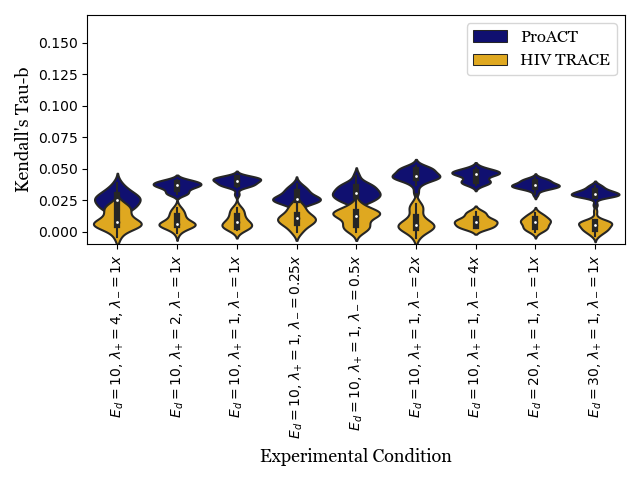
\includegraphics[scale=0.5]{Figures/m1_tau_updated.png}
% \caption{Metric 1: A violin plot showing the results of SEPIA on HIV-Trace and ProACT over simulated data with different conditions. All conditions receive a correlation coefficient above, but still close to, zero. Thus, it shows that both algorithms create orderings which are close to random compared to the optimal ordering generated by the metric. \cite{wertheim2018growth, moshiri2019ProACT}.} 
% \end{figure}

% \begin{figure}[h!]  %Figure 7
% \centering
% \title\textbf{Metric 2}\par\medskip
% 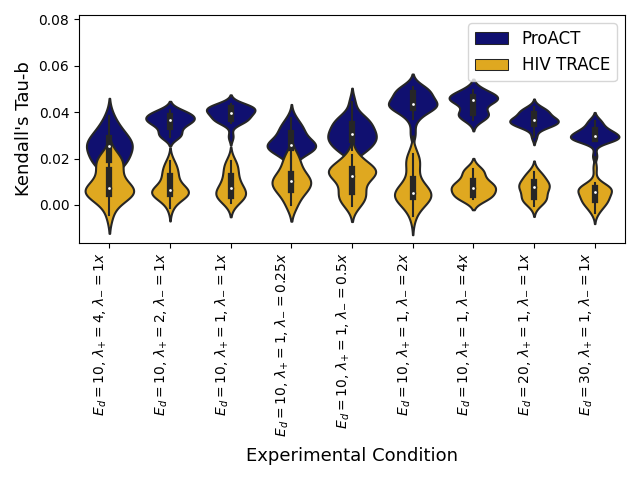
\includegraphics[scale=0.5]{Figures/m2_tau.png}
% \caption{Metric 2: A violin plot showing the results of SEPIA on HIV-Trace and ProACT over simulated data with different conditions. All conditions receive a correlation coefficient above, but still close to, zero. Thus, it shows that both algorithms create orderings which are close to random compared to the optimal ordering generated by the metric. \cite{wertheim2018growth, moshiri2019ProACT}.} 
% \end{figure}

% \begin{figure}[h!] %Figure 8
% \centering
% \title\textbf{Metric 3}\par\medskip
% 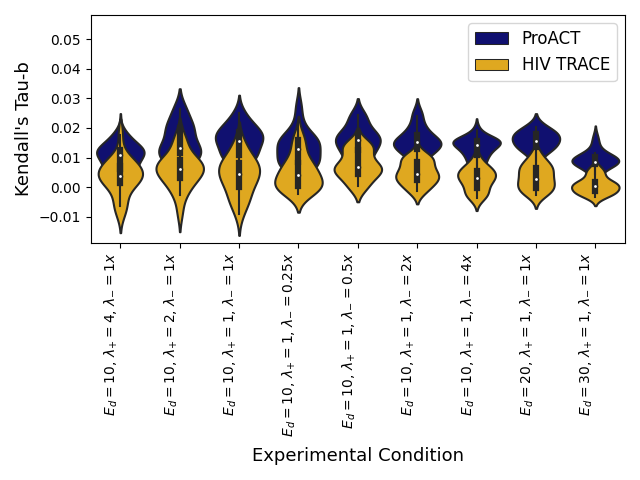
\includegraphics[scale=0.5]{Figures/m3_tau.png}
% \caption{Metric 3: A violin plot showing the results of SEPIA on HIV-Trace and ProACT over simulated data with different conditions. All conditions receive a correlation coefficient above, but still close to, zero. Thus, it shows that both algorithms create orderings which are close to random compared to the optimal ordering generated by the metric. \cite{wertheim2018growth, moshiri2019ProACT}.} 
% \end{figure}

% \begin{figure}[h!] %Figure 9
% \centering
% \title\textbf{Metric 4}\par\medskip
% 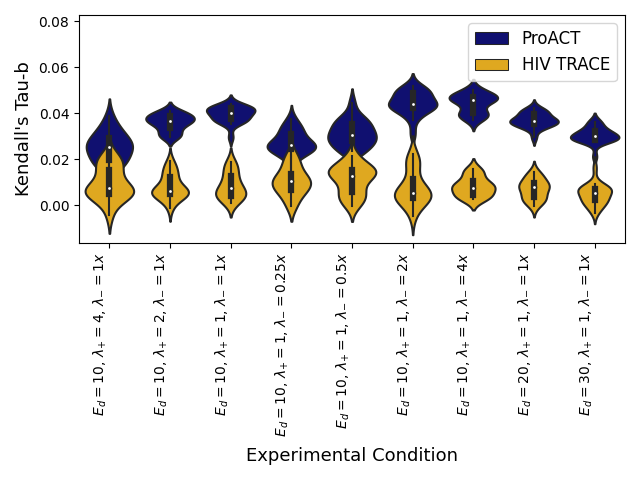
\includegraphics[scale=0.5]{Figures/m4_tau.png}
% \caption{Metric 4: A violin plot showing the results of SEPIA on HIV-Trace and ProACT over simulated data with different conditions. All conditions receive a correlation coefficient above, but still close to, zero. Thus, it shows that both algorithms create orderings which are close to random compared to the optimal ordering generated by the metric. \cite{wertheim2018growth, moshiri2019ProACT}.} 
% \end{figure}

% \begin{figure}[h!] %Figure 10
% \centering
% \title\textbf{Metric 5}\par\medskip
% 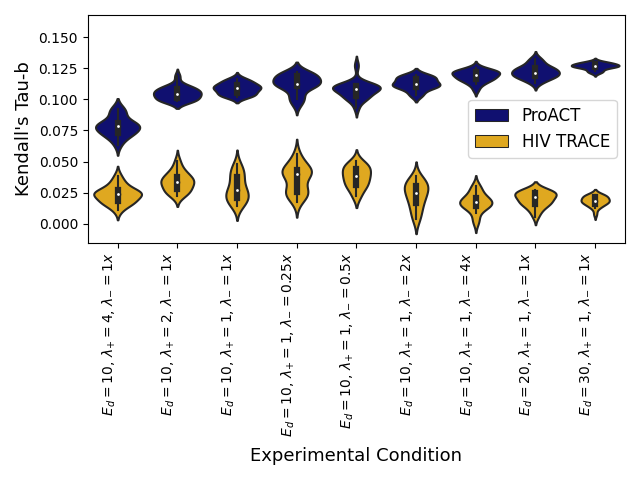
\includegraphics[scale=0.5]{Figures/m5_tau.png}
% \caption{Metric 5: A violin plot showing the results of SEPIA on HIV-Trace and ProACT over simulated data with different conditions. All conditions receive a correlation coefficient above, but still close to, zero. Thus, it shows that both algorithms create orderings which are close to random compared to the optimal ordering generated by the metric. \cite{wertheim2018growth, moshiri2019ProACT}.} 
% \end{figure}

% \begin{figure}[h!] %Figure 11
% \centering
% \title\textbf{Metric 6}\par\medskip
% 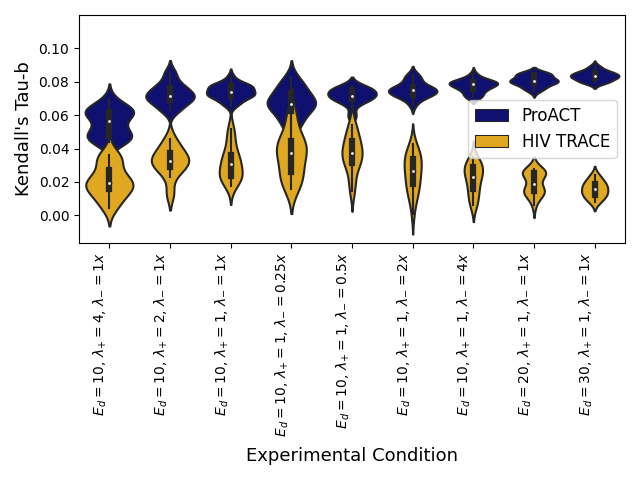
\includegraphics[scale=0.5]{Figures/m6_tau.png}
% \caption{Metric 6: A violin plot showing the results of SEPIA on HIV-Trace and ProACT over simulated data with different conditions. All conditions receive a correlation coefficient above, but still close to, zero. Thus, it shows that both algorithms create orderings which are close to random compared to the optimal ordering generated by the metric. \cite{wertheim2018growth, moshiri2019ProACT}.} 
% \end{figure}


\begin{figure*}[p!]  %Figure 3
\centering
\title\par\medskip
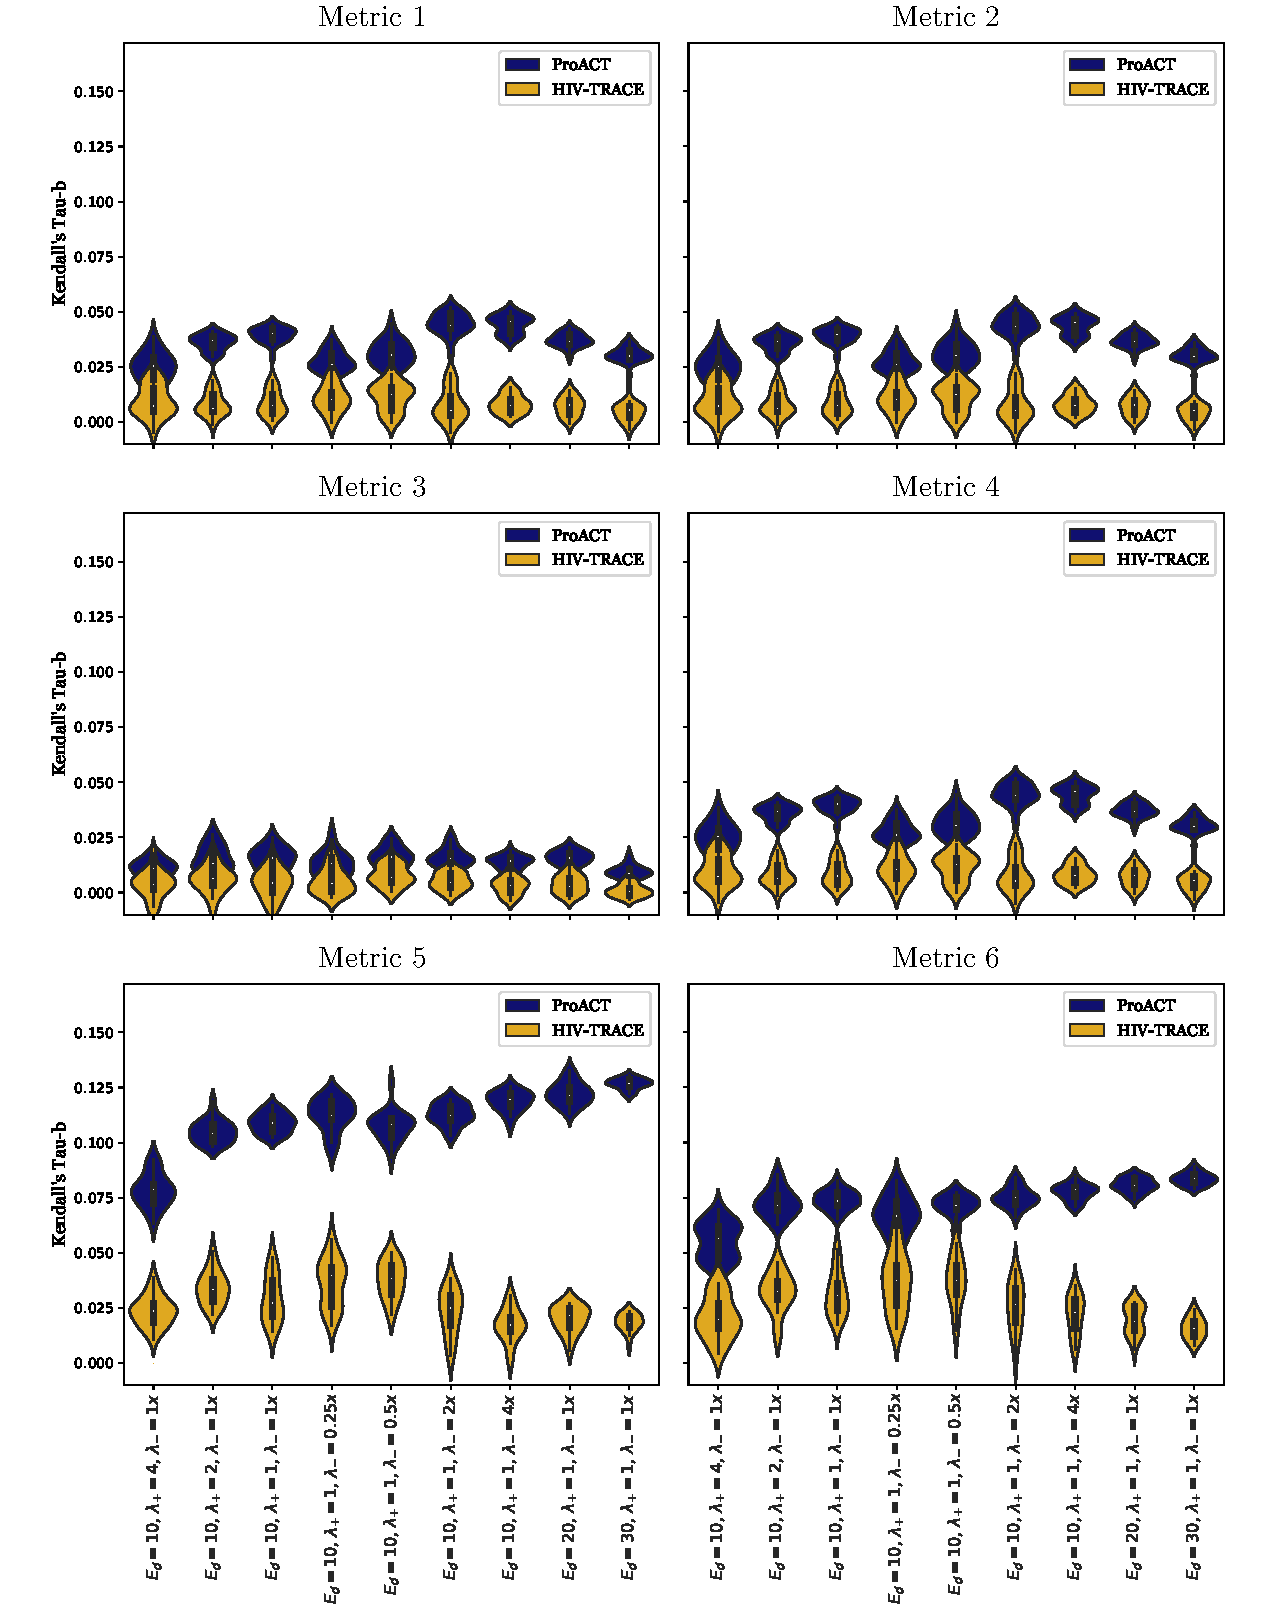
\includegraphics[width=0.95\textwidth]{Figures/Fig3.pdf}
\caption{Efficacy of ProACT and HIV-TRACE across all metrics on datasets simulated by FAVITES. The violin plots depict the Kendall Tau-b correlation coefficients between experimental and optimal orderings across 20 replicates for each experimental condition. The experimental conditions are varied by altering 3 parameters, where $E_d$ denotes the expected number of contacts per individual, $\lambda_+$ denotes the rate at which individuals begin ART, and $\lambda_-$ denotes the rate at which individuals stop ART.
} 
\end{figure*}
%%%%%%%%%%%%%%%%%%%%%%%%%%%%%%%%%%%%%%%%%%%%%%
%%                                          %%
%% Backmatter begins here                   %%
%%                                          %%
%%%%%%%%%%%%%%%%%%%%%%%%%%%%%%%%%%%%%%%%%%%%%%

\begin{backmatter}

\section*{Competing interests}
  The authors declare that they have no competing interests.

\section*{Author's contributions}
    NM conceived and directed this project. All members wrote the code for this project. KA, TJ, ML, TN, MS and NM composed this manuscript.
    
\section*{Acknowledgements}
 We would like to acknowledge the Early Research Scholars Program organized by Professor Christine Alvarado and Vignesh Gokul at the University of California, San Diego for granting us this opportunity.
  
\section*{Availability of data and materials}
SEPIA can be found as an open source tool at: \href{https://github.com/Niema-Lab/SEPIA}{https://github.com/Niema-Lab/SEPIA}

The simulated data can be found at: \href{https://github.com/Niema-Lab/SEPIA-paper-final}{https://github.com/Niema-Lab/SEPIA-paper-final}

\section*{Consent for publication}
    Not Applicable.
    
\section*{Ethics approval and consent to participate}
    Not Applicable.
    
\section*{Author Information}
    Department of Computer Science and Engineering, University of California San Diego, 9500 Gilman Drive, La Jolla, CA, 92093, USA
    \newline
    Kimberly Almaraz, Tyler Jang, McKenna Lewis, Titan Ngo, Miranda Song and Niema Moshiri
    
%%%%%%%%%%%%%%%%%%%%%%%%%%%%%%%%%%%%%%%%%%%%%%%%%%%%%%%%%%%%%
%%                  The Bibliography                       %%
%%                                                         %%
%%  Bmc_mathpys.bst  will be used to                       %%
%%  create a .BBL file for submission.                     %%
%%  After submission of the .TEX file,                     %%
%%  you will be prompted to submit your .BBL file.         %%
%%                                                         %%
%%                                                         %%
%%  Note that the displayed Bibliography will not          %%
%%  necessarily be rendered by Latex exactly as specified  %%
%%  in the online Instructions for Authors.                %%
%%                                                         %%
%%%%%%%%%%%%%%%%%%%%%%%%%%%%%%%%%%%%%%%%%%%%%%%%%%%%%%%%%%%%%

% if your bibliography is in bibtex format, use those commands:
\bibliographystyle{bmc-mathphys} % Style BST file (bmc-mathphys, vancouver, spbasic).
\bibliography{bmc_article}      % Bibliography file (usually '*.bib' )
% for author-year bibliography (bmc-mathphys or spbasic)
% a) write to bib file (bmc-mathphys only)
% @settings{label, options="nameyear"}
% b) uncomment next line
%\nocite{label}

% or include bibliography directly:
% \begin{thebibliography}
% \bibitem{b1}
% \end{thebibliography}

%%%%%%%%%%%%%%%%%%%%%%%%%%%%%%%%%%%
%%                               %%
%% Figures                       %%
%%                               %%
%% NB: this is for captions and  %%
%% Titles. All graphics must be  %%
%% submitted separately and NOT  %%
%% included in the Tex document  %%
%%                               %%
%%%%%%%%%%%%%%%%%%%%%%%%%%%%%%%%%%%

%%
%% Do not use \listoffigures as most will included as separate files
%%
%\section*{Figures}
%%  \begin{figure}[H]
%  \caption{\csentence{Sample figure title.}
%      A short description of the figure content
%      should go here.}
%      \end{figure}
%
%\begin{figure}[H]
%  \caption{\csentence{Sample figure title.}
%      Figure legend text.}
%      \end{figure}

%%%%%%%%%%%%%%%%%%%%%%%%%%%%%%%%%%%
%%                               %%
%% Tables                        %%
%%                               %%
%%%%%%%%%%%%%%%%%%%%%%%%%%%%%%%%%%%

%% Use of \listoftables is discouraged.
%%
%\section*{Tables}
%\begin{table}[H]
%\caption{Sample table title. This is where the description of the table should %go.}
%      \begin{tabular}{cccc}
%        \hline
%           & B1  &B2   & B3\\ \hline
%        A1 & 0.1 & 0.2 & 0.3\\
%        A2 & ... & ..  & .\\
%        A3 & ..  & .   & .\\ \hline
%      \end{tabular}
%%end{table}

%%%%%%%%%%%%%%%%%%%%%%%%%%%%%%%%%%%
%%                               %%
%% Additional Files              %%https://www.overleaf.com/project/5efbdbb0b78c5f00018e8a23
%%                               %%
%%%%%%%%%%%%%%%%%%%%%%%%%%%%%%%%%%%
%%
%\section*{Additional Files}
%  \subsection*{Additional file 1 --- Sample additional file title}
%    Additional file descriptions text (including details of how to
%    view the file, if it is in a non-standard format or the file extension).  %This might
%    refer to a multi-page table or a figure.
%
%  \subsection*{Additional file 2 --- Sample additional file title}
%    Additional file descriptions text.


\end{backmatter}
\end{document}

